\chapter{Introduction}\label{ch:introduction}


Graph representation has gained wide popularity as a data representation method in many applications. Graph embedding methods convert graphs to a vector representation and are an important part of a data processing pipeline. In this paper, we utilize sparse dictionary learning techniques as a graph embedding solution. Sparse representation has notable applications in signal image processing. Inspired by the Graph2Vec algorithm, we aim to modify the Doc2Vec model training portion of the Graph2Vec by incorporating unsupervised dictionary learning. We investigate the viability of using the sparse dictionary learning technique KSVD for graph data. We train the dictionary on Weisfeiler-Lehman graph sub-tree kernel features. Furthermore, we use graph-based labeled data sets to compare classification results with several existing graph embedding methods. Findings show that using the learned sparse coefficients as features for a supervised machine learning algorithm provides on-par classification results when compared to other graph embedding methods. 

\section{Motivation}

\section{Goals and Objectives}

\subsection{Goal}

\subsection{Objective}
A Graph is represented as one sparse vector and two graphs with similar sub- structure are embedded to be closer.

The Graph can be
\begin{itemize}
    \item Directed
    \item Cyclic
    \item Have node feature
\end{itemize}

\begin{enumerate}
    \item To develop a sub-tree pattern based sparse graph embedding method
    \item Framework for Identifying important sub-tree patterns
    \item Develop  a sparse graph representation in hyperbolic space
\end{enumerate}

\begin{figure}[!tbh]
    \centering
    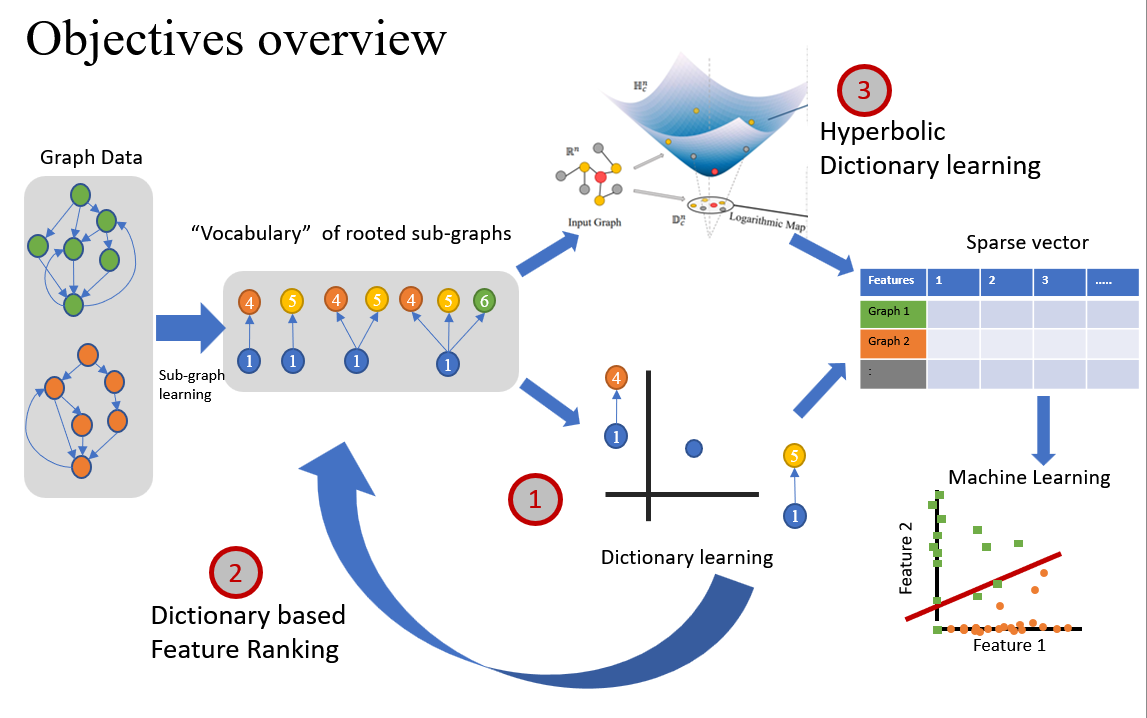
\includegraphics[width=\columnwidth]{figures/presentation/Objective_overview.png}
    \caption[overview]{The proposal objectives overview}\label{fig:obj_overview}
\end{figure}